\subsection{Análise anual}
Inicialmente, foram levantadas as quantidades de ligações registradas durante o ano e a quantidade total de falhas, assim como o percentual de falhas. No ano de 2021, que contou com 261 dias de trabalho, foram registradas 51.708 ligações, sendo que 4.227 destas demoraram mais de 60 segundos para serem atendidas, caracterizando falha do processo. O percentual destas falhas para o ano foi de 8,17\%, valor que atende as especificações de desempenho da empresa. No entanto, como este valor representa apenas uma média anual, devemos buscar compreender o problema da empresa ao avaliar o comportamento das variáveis relevantes do processo ao longo do ano.

\subsubsection{Quantidade de chamados por dia}
A Figura \ref*{fig: chamados-tempo} apresenta a quantidade de chamadas recebidas por dia ao longo do ano. É possível perceber uma relação de dependência entre a quantidade de ligações recebidas e os dias do ano, visto que o número de chamadas cresce ao longo do ano. Esse comportamento pode ser responsável pelo aumento do percentual de falhas em meses próximos ao fim do ano. Posteriormente, será descrito um estudo de regressão para estes dados.

\begin{figure}[H]
    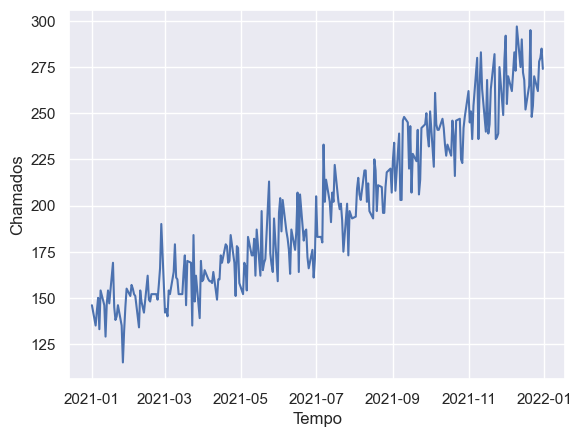
\includegraphics{analise-de-dados/anual/chamados.png}
    \caption{Quantidade de chamadas recebidas ao longo do tempo}
    \label{fig: chamados-tempo}
\end{figure}

\subsubsection{Análise e descrição dos tempos de espera e serviço}
Como os tempos de espera (\textit{wait length}) e serviço (\textit{service length}) já estão calculados, podemos analisar seu comportamento. A Tabela \ref*{tab: descricao-serviço-espera} apresenta as estatísticas descritivas dos tempos de espera e dos tempos de serviço. É notável que a maioria dos tempos de espera (pelo menos 75\% deles) são nulos, e a média fica abaixo dos 60 segundos, no entanto, o valor máximo é muito elevado. O tempo de serviço também apresenta um valor máximo distante da média.

\begin{table}[H]
\centering
    \begin{tabular}{lr}
        % \begin{center}
            \toprule
            {} &  Tempo de espera \\
            \midrule
            count &   51708.000  \\
            mean  &      17.035  \\
            std   &      64.061  \\
            min   &       0.000  \\
            25\%   &       0.000  \\
            50\%   &       0.000  \\
            75\%   &       0.000  \\
            max   &     983.000  \\
        % \end{center}
        \bottomrule
        % \label{tab: describe-wait}
    \end{tabular}
    \quad
    \begin{tabular}{lr}
        % \begin{center}
            \toprule
            {} &  Tempo de serviço \\
            \midrule
            count &     51708.000   \\
            mean  &       299.103   \\
            std   &       299.866   \\
            min   &         0.000   \\
            25\%   &        86.000   \\
            50\%   &       208.000   \\
            75\%   &       414.000   \\
            max   &      3110.000   \\
        % \end{center}
        \bottomrule
        % \label{tab: describe-wait}
    \end{tabular}
    \caption{Estatística descritiva dos tempos de espera e de serviço}
    \label{tab: descricao-serviço-espera}
\end{table}

Para visualizar a distribuição dos valores estudados, foram criados boxplots. A Figura \ref*{fig: box-wait} mostra o boxplot para a variável de tempos de espera apresentando outliers moderados. A Figura \ref*{fig: box-time} é o boxplot dos tempos de serviço e seus outliers moderados. Em nossa análise, decidimos não retirar os outliers, pois é interessante para o problema a modelagem de variáveis aleatórias com distribuições que levem em consideração a presença de valores extremos (caudas longas).

\begin{figure}[H]
    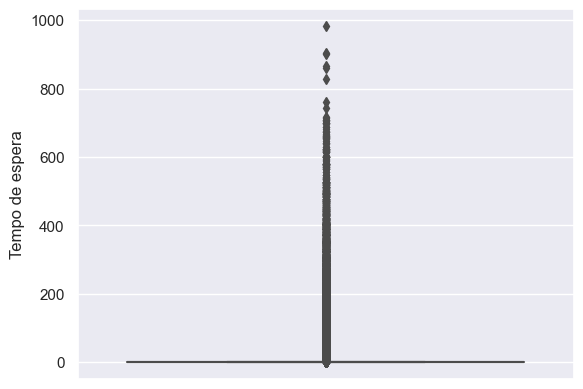
\includegraphics{analise-de-dados/anual/box-wait.png}
    \caption{Boxplot tempos de espera}
    \label{fig: box-wait}
\end{figure}

\begin{figure}[H]
    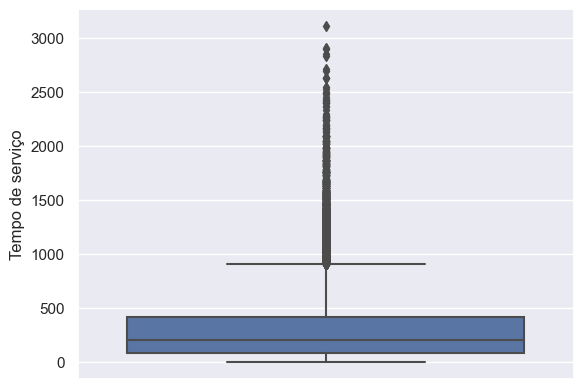
\includegraphics{analise-de-dados/anual/box-service.png}
    \caption{Boxplot tempos de serviço}
    \label{fig: box-time}
\end{figure}

O comportamento do tempo médio de serviço ao longo do ano pode ser visto na Figura \ref*{fig: t_servico-tempo} e apresenta um caráter permanente.

\begin{figure}[H]
    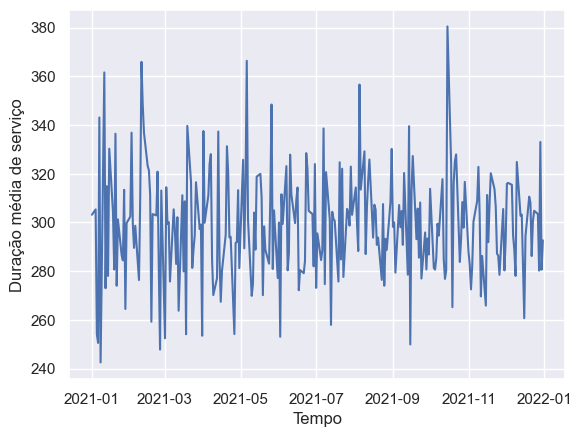
\includegraphics{analise-de-dados/anual/service_len.png}
    \caption{Tempos médios de serviço ao longo do tempo}
    \label{fig: t_servico-tempo}
\end{figure}

Para testar a hipótese que o tempo de serviço segue uma mesma distribuição ao longo do ano, foi utilizado o teste não paramétrico de Kolgomorov-Smirnov com duas amostras, testando os meses dois a dois. Os resultados estão na Figura \ref*{fig: KS_servico}. As células em verde possuem valor $p$ maior que o nível de significância adotado que é $\alpha = 5\%$, e, portanto, não há diferenças estatisticamente significativas entre a distribuição dos tempos de serviço ao longo dos meses do ano.

\begin{figure}[H]
    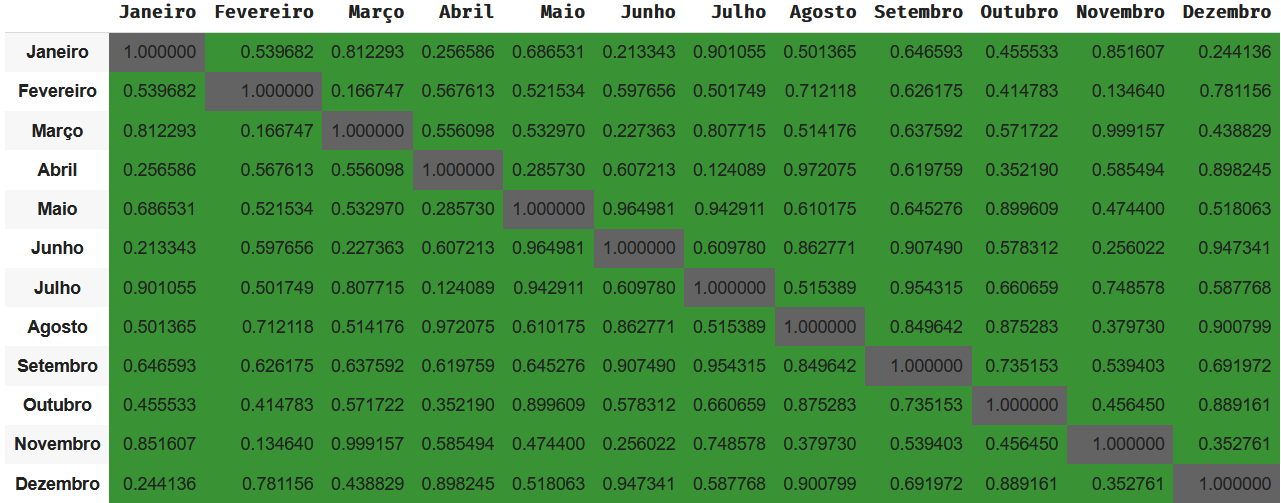
\includegraphics[scale=0.6]{analise-de-dados/anual/ks-service.png}
    \caption{$p$ valores do teste KS 2 amostras para tempos de serviço}
    \label{fig: KS_servico}
\end{figure}

O tempo médio de espera ao longo do ano é representado na Figura \ref*{fig: espera-tempo}. A Figura \ref*{fig: KS_wait} mostra o teste de hipóteses para os tempos de espera mês a mês. É possível concluir que no início do ano (até o mês de maio), não houve diferenças significativas entre os tempos de espera. No entanto, a partir de junho, é possível atestar diferenças mais acentuadas na distribuição dos tempos de espera, representado pelos $p$ valores abaixo de 5\%, apresentado pelas células em vermelho.

\begin{figure}[H]
    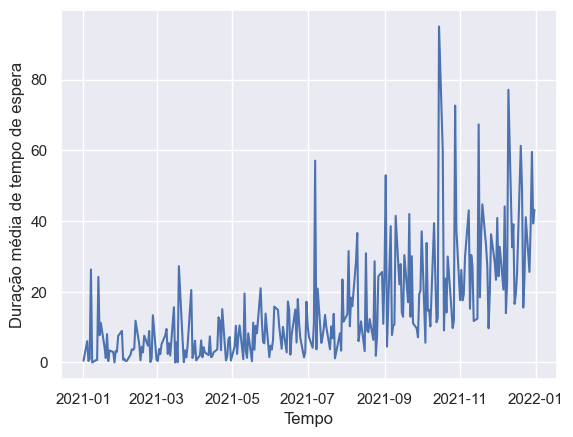
\includegraphics{analise-de-dados/anual/service.png}
    \caption{Tempos médios de espera ao longo do ano}
    \label{fig: espera-tempo}
\end{figure}

\begin{figure}[H]
    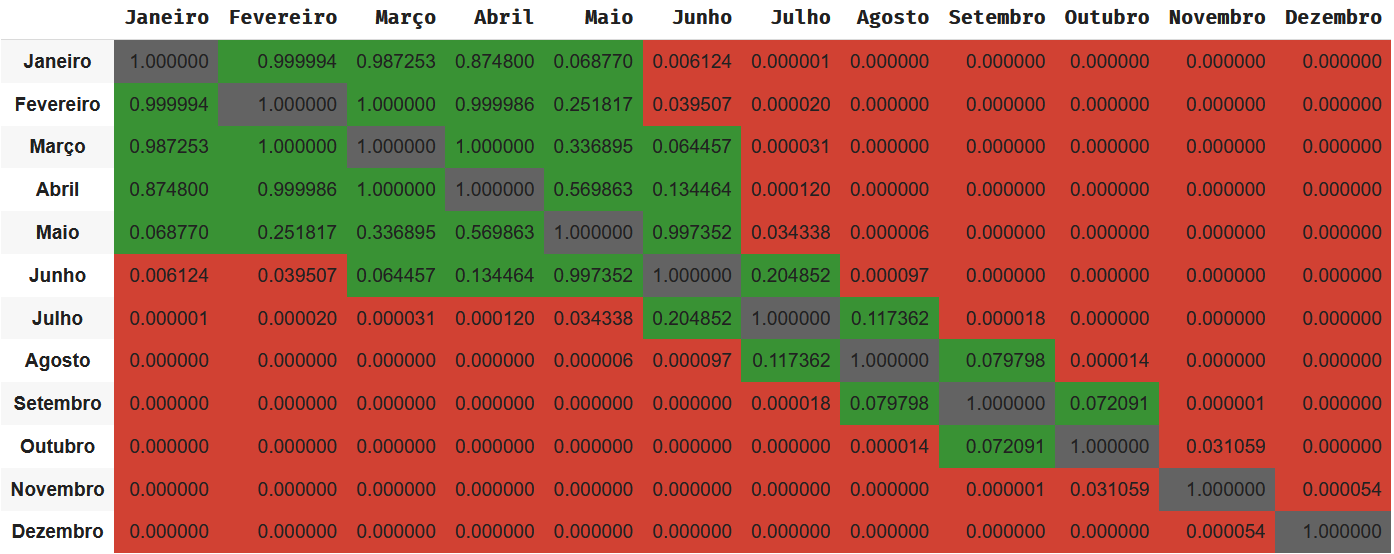
\includegraphics[scale=0.55]{analise-de-dados/anual/ks-wait.png}
    \caption{$p$ valores do teste KS 2 amostras para tempos de espera}
    \label{fig: KS_wait}
\end{figure}

\subsubsection{Fit dos tempos serviços}
A Figura \ref*{fig: hist-servicos} apresenta o histograma dos tempos de serviço. O formato se assemelha ao de uma distribuição exponencial. Para testar a aderência de distribuições de probabilidade a essa variável aleatória é utilizada a biblioteca Fitter do Python que testa para algumas distribuições comuns utilizando o teste de Kolgomorov-Smirnov. A partir da Figura \ref*{fig: fit-servicos}, ao escolhermos a distribuição de menor erro quadrado, concluímos que o tempo de serviço pode ser modelado por uma distribuição exponencial de média 299,1 segundos. Não foi realizada modelagem dos tempos de espera, visto que estes não possuem duração definida e não são necessários para modelagem posterior.

\begin{figure}[H]
    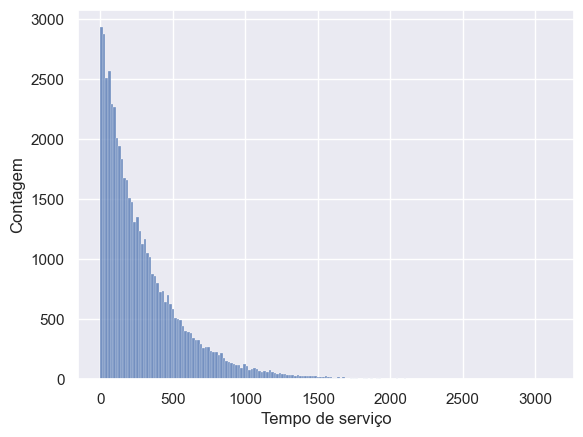
\includegraphics{analise-de-dados/anual/histograma-servicos.png}
    \caption{Histograma dos tempos de serviço}
    \label{fig: hist-servicos}
\end{figure}

\begin{figure}[H]
    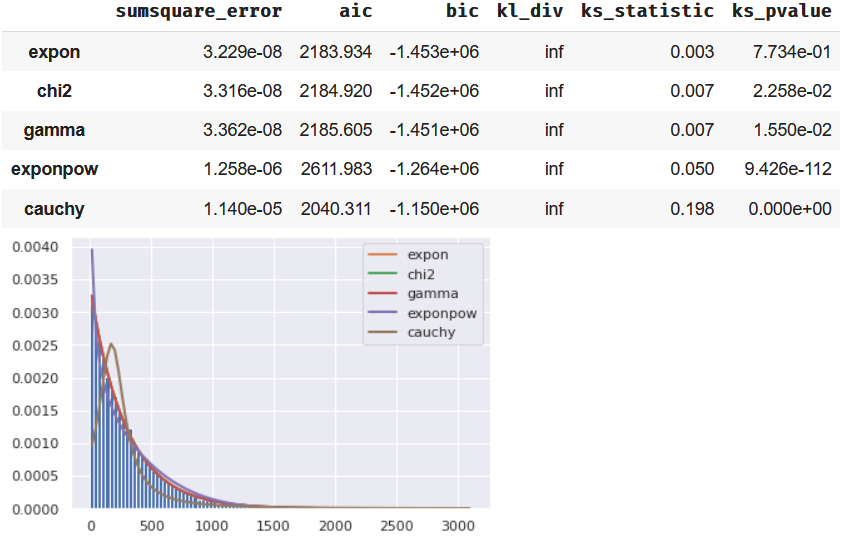
\includegraphics[scale=.9]{analise-de-dados/anual/fit-servicos.png}
    \caption{Fit dos dados às distribuições de probabilidade}
    \label{fig: fit-servicos}
\end{figure}

\subsubsection{Análise dos tempos entre chegadas das ligações}
Para modelar os intervalos entre chegadas no Arena é necessário subtrair os intervalos entre chegadas das ligações em um mesmo dia. Dessa operação resulta a coluna "arrival\_time\_diff", na Figura \ref*{fig: df-intervalos}, que é colocada na base de dados. \\
O histograma dos intervalos de chegada na Figura \ref*{fig: hist-intervalos} também se assemelha a uma distribuição exponencial.

\begin{figure}[H]
    \centering
    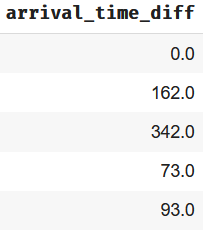
\includegraphics{analise-de-dados/anual/df-arrivals.png}
    \caption{Coluna de intervalos entre chegadas - 5 primeiros valores}
    \label{fig: df-intervalos}
\end{figure}

\begin{figure}[H]
    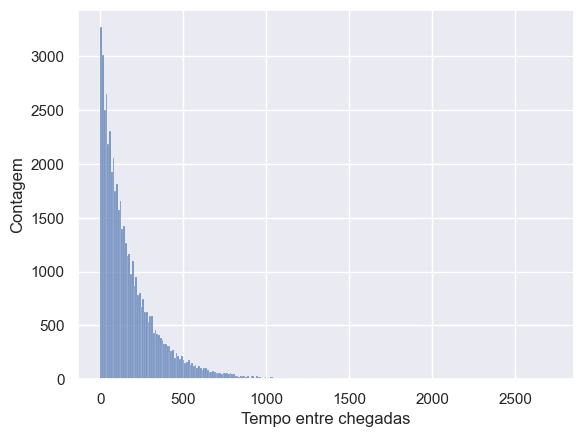
\includegraphics{analise-de-dados/anual/hist-intervalos.png}
    \caption{Histograma dos intervalos entre chegadas}
    \label{fig: hist-intervalos}
\end{figure}

A Figura \ref*{fig: arrivals-tempo} apresenta a variável de intervalo entre chegadas ao longo do ano, que demonstra tendência de queda com o passar do tempo. Essa observação está de acordo com a Figura \ref*{fig: chamados-tempo} que mostra aumento do número de ligações ao longo do ano. 

\begin{figure}[H]
    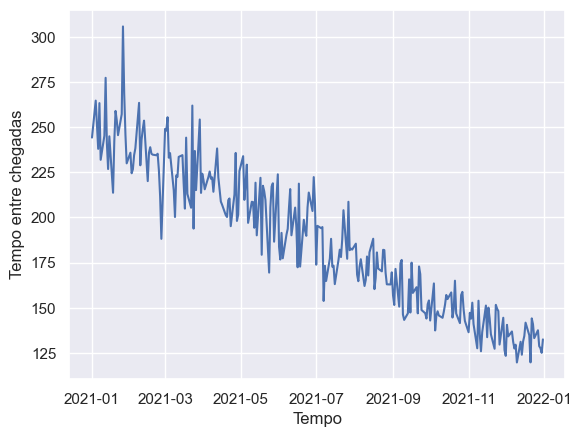
\includegraphics{analise-de-dados/anual/arrivals-tempo.png}
    \caption{Tempo entre chegadas ao longo do tempo}
    \label{fig: arrivals-tempo}
\end{figure}

É interessante notar que mesmo para meses subsequentes, o teste de Kolgomogorov-Smirnov de 2 amostras resumido na Figura \ref*{fig: ks-arrivals} rejeita a hipótese de que a distribuição dos tempos de chegada entre eles seja idêntica. Isso indica que não é viável agregar períodos maiores que um mês para modelagem das chegadas. Os valores em vermelho são aqueles nos quais o teste rejeitou a hipótese nula, e, portanto, há diferenças significativas de distribuições de probabilidade entre os meses. Portanto, não é viável modelar a variável de intervalo entre chegadas utilizando uma única distribuição de probabilidade para todo o ano.\\
A Tabela \ref*{tab: descricao-arrivals} apresenta a estatística descritiva desses intervalos entre chegadas.

\begin{figure}[H]
    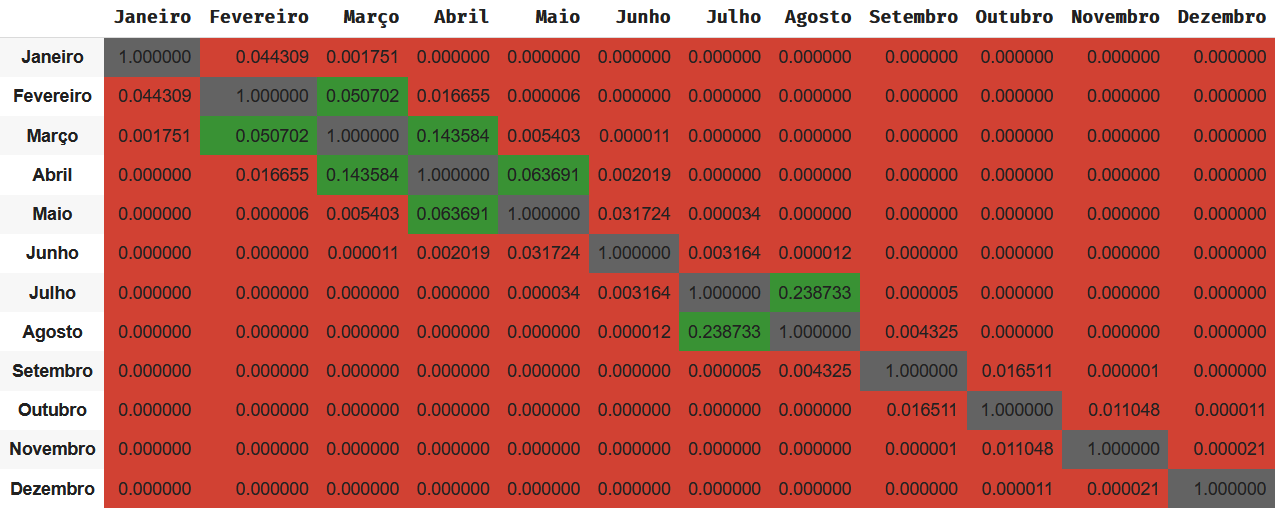
\includegraphics[scale=0.6]{analise-de-dados/anual/ks-arrivals.png}
    \caption{$p$ valores do teste KS 2 amostras para tempos de serviço}
    \label{fig: ks-arrivals}
\end{figure}

\begin{table}[H]
    \centering
    \begin{tabular}{lr}
        % \begin{center}
            \toprule
            {} &  Intervalos entre chegadas \\
            \midrule
            count &   51708.000  \\
            mean  &      179.668  \\
            std   &      188.007  \\
            min   &       0.000  \\
            25\%   &       49.000  \\
            50\%   &       121.000  \\
            75\%   &       246.000  \\
            max   &     2718.000  \\
        \bottomrule
        \end{tabular}
    \caption{Estatística descritiva dos tempos entre chegadas}
    \label{tab: descricao-arrivals}
\end{table}

\subsubsection{Teste de correlação entre os tempos estudados}
Para testar a correlação utilizamos a correlação de Spearman, por se tratar de um teste não paramétrico, visto que estamos trabalhando com variáveis que não seguem a distribuição normal. A Figura \ref*{fig: corr-spearman-1} mostra os coeficientes de correlação obtidos.\\
A Figura \ref*{fig: spearman-test-1} contém os $p$ valores do teste de correlação de Spearman para as variáveis aleatórias estudadas. Como a hipótese nula do teste é que não há correlação, temos rejeição da hipótese nula apenas para a correlação entre os intervalos de chegada ("arrival\_time\_diff") e os tempos de espera ("wait\_length"), com valor $p$ menor que 5\%. Assim, como o tempo de serviço não varia ao longo do ano, o aumento do tempo de espera é explicado pela redução do intervalo entre chegadas, e pelo consequente aumento do número de chamadas diário ao longo do ano.

\begin{figure}[H]
    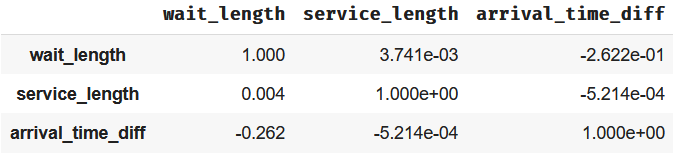
\includegraphics{analise-de-dados/anual/corr-spearman.png}
    \caption{Coeficientes de correlação de Spearman entre os tempos}
    \label{fig: corr-spearman-1}
\end{figure}

\begin{figure}[H]
    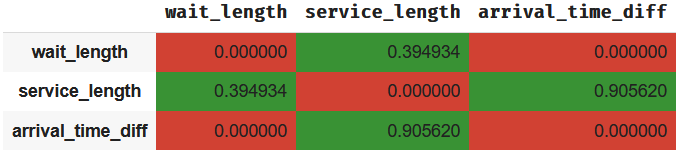
\includegraphics{analise-de-dados/anual/spearman-test.png}
    \caption{Testes de correlação entre as variáveis}
    \label{fig: spearman-test-1}
\end{figure}

\subsection{Análise dos call types}
A base de dados conta com uma coluna "call\_types", com os valores 0, 1 e 2, que identificam diferentes categorias de ligações. É interessante estudar a relação entre esses tipos para identificar possíveis diferenças na distribuição dos tempos de interesse entre eles. A Tabela \ref*{tab: call-type} avalia as ligações recebidas por tipo em base anual. O tipo de ligação 1 é, em média, duas vezes mais frequente que os outros dois tipos, no entanto, o percentual de falhas entre eles não é muito diferente, sendo as falhas definidas como as ligações que não atenderam os requisitos de tempo de espera inferior a 60 segundos.

\begin{table}[H]
    \centering
    \begin{tabular}{|l|r|r|r|}
    \hline
    \textbf{Call type} & 0 & 1 & 2 \\ \hline
    Quantidade & 12830 & 25792 & 13086 \\ \hline
    Falhas & 1069 & 2100 & 1058 \\ \hline
    Percentual de falhas & 8,33\% & 8,14\% & 8,08\% \\ \hline
    \end{tabular}
    \caption{Status de ligações por tipo}
    \label{tab: call-type}
\end{table}
    
Foram realizados testes de Kolgomorov-Smirnov para testar a hipótese de que, para cada um dos três tipos, não há diferenças significativas entre os tempos de interesse. A Figura \ref*{fig: KS_tipos_servico} mostra os valores $p$ do teste entre os tipos para a variável aleatória de tempo de serviço. A Figura \ref*{fig: KS_tipos_chegada} mostra os valores $p$ do teste entre os tipos para a variável de tempo de chegada. Por fim, a Figura \ref*{fig: KS_tipos_espera} mostra os valores $p$ do teste entre os tipos para a variável de tempo de espera. Portanto, não houve diferença estatística entre as distribuições dos tempos de chegada, de serviço e de espera de acordo com o tipo de ligação em base anual, ja que a hipótese nula de que os valores seguem a mesma distribuição não foi rejeitada em nenhum teste.

\begin{figure}[H]
    \centering
    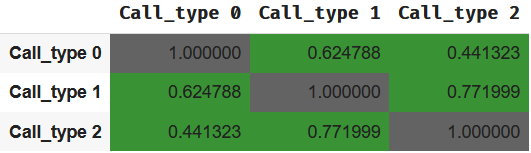
\includegraphics{analise-de-dados/anual/ks-tipos-service.png}
    \caption{$p$ valores do teste KS 2 amostras para tempos de serviço para cada tipo de ligação}
    \label{fig: KS_tipos_servico}
\end{figure}

\begin{figure}[H]
    \centering
    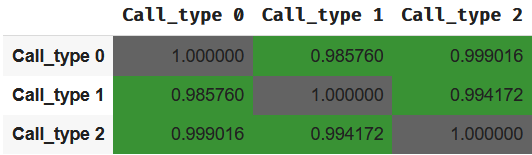
\includegraphics{analise-de-dados/anual/ks-tipos-chegadas.png}
    \caption{$p$ valores do teste KS 2 amostras para intervalos de chegada para cada tipo de ligação}
    \label{fig: KS_tipos_chegada}
\end{figure}

\begin{figure}[H]
    \centering
    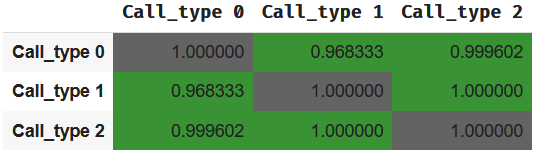
\includegraphics{analise-de-dados/anual/ks-tipos-espera.png}
    \caption{$p$ valores do teste KS 2 amostras para tempos de espera para cada tipo de ligação}
    \label{fig: KS_tipos_espera}
\end{figure}
